% !TeX root = ../../../book.tex

\subsection{乘法原理}

\subsubsection*{引言}

我们通过一个例子来引出乘法原理。\\

\begin{example}
    假设房间里有三个人和三张贴纸,分别标有数字 $1, 2, 3$。我们有多少种方法可以将这些贴纸分配给这三个人?为了方便讨论,假设这三个人分别叫 Andy、Brendan 和 Carl,简称 $A, B, C$。我们可以有条理地列出所有可能的贴纸分配方式,以确保不遗漏任何一种情况。具体来说,我们会让 Andy 先选,然后是 Brendan,再然后是 Carl:我们有 $(A, B, C) = $
    \begin{itemize}
        \item $(1, 2, 3)$
        \item $(1, 3, 2)$
        \item $(2, 1, 3)$
        \item $(2, 3, 1)$
        \item $(3, 1, 2)$
        \item $(3, 2, 1)$
    \end{itemize}
    因此,总共有 $6$ 种贴纸分配方案。

    如果我们有四个人 --- Andy、Brendan、 Carl 和 Dave ---和四张贴纸呢?我们能列出所有贴纸分配方案吗?当然可以。
    \begin{align*}
        (1, 2, 3, 4) \quad (1, 2, 4, 3) \quad (1, 3, 2, 4) \quad (1, 3, 4, 2) \\
        (1, 4, 2, 3) \quad (1, 4, 3, 2) \quad (2, 1, 3, 4) \quad (2, 1, 4, 3) \\
        (2, 3, 1, 4) \quad (2, 3, 4, 1) \quad (2, 4, 1, 3) \quad (2, 4, 3, 1) \\
        (3, 1, 2, 4) \quad (3, 1, 4, 2) \quad (3, 2, 1, 4) \quad (3, 2, 4, 1) \\
        (3, 4, 1, 2) \quad (3, 4, 2, 1) \quad (4, 1, 2, 3) \quad (4, 1, 3, 2) \\
        (4, 2, 1, 3) \quad (4, 2, 3, 1) \quad (4, 3, 1, 2) \quad (4, 3, 2, 1)
    \end{align*}
    所以总共有 $24$ 种贴纸分配方案。那五个人呢?我不知道你怎么样,反正我写这么多分配方案已经写得胳膊酸了。一定有更好的方法来完成这件事!没错!这时就需要乘法原理出马了。(旁注:你可能注意到我们上面的列表有一定规律;你能推断出我们是如何确保列出了所有可能性吗?你能写一个小程序对于任意输入人数生成所有可能性吗?试试看吧!)
\end{example}

\subsubsection*{陈述}

实际上我们会对乘法原理做出两个独立的陈述。第一个是关于何时以及如何应用的直观陈述。第二个是基于集合论语言的更为严格的数学陈述。这里强调一点,理想情况下这两个陈述都需要理解;但相比之下理解第一个更加重要,因为第二个主要是为了能够进行严格证明。

\begin{proposition}
    考虑一个由 $n$ 个独立步骤组成的过程。假设第 $i$ 步,对于每个 $i \in [n]$,有恰好有 $w_i$ 种不同的完成方式;并且假设这个数量 $w_i \in \mathbb{N}$ 不依赖于前一步所做的选择。同时,假设在任何一步中,每个不同的选择都会产生不同的结果。那么乘法原理表明,这个由 $n$ 个步骤组成的过程的总结果数 $N$ 为
    \[N = \prod_{i \in [n]} w_i\]
\end{proposition}

在更加严谨地阐述乘法原理之前,让我们先回顾一下之前分配贴纸的例子。\\

\begin{example}
    我们可以将给 Andy、Brendan 和 Carl 分配贴纸看作一个三步过程。首先,我们按字母顺序从左到右将三人排序,然后依次给他们贴上贴纸。每一步中,我们选择一个尚未分配的贴纸贴在此人身上。

    第一步,我们来到 Andy 面前,有 $3$ 种贴纸可以选择。

    第二步,我们来到 Brendan 面前,此时有 $2$ 种贴纸可以选择。注意,无论我们前面给 Andy 选择了哪种贴纸,这个数量都是不变的。我们不在乎给 Andy 选择了 $1$ 还是 $2$ 抑或是 $3$,只要面对 Brendan 时,我们总有 $2$ 种选择。

    第三步,我们来到 Carl 面前,无论前两步选择了什么,我们都只剩 $1$ 种贴纸可以选择。

    乘法原理告诉我们,完成这个过程的方法数量是每一步选择数量的乘积:$3 \cdot 2 \cdot 1 = 6$。这与我们``穷举所有可能''的方法一致。太棒了!

    如果是 $4$ 个人呢?使用相同的逻辑,我们可以看到,完成贴纸分配过程的方法有 $4 \cdot 3 \cdot 2 \cdot 1 = 24$。这也与我们之前列出的结果一致。太棒了!

    如果是 $5$ 个人呢?那么,$5 \cdot 4 \cdot 3 \cdot 2 \cdot 1 = 120$。我们发现了一个新的结果。真是太惊喜了!如果是 $6$ 个人呢?如果是 $7$ 个人呢?如果是 $n$ 个人,其中 $n \in \mathbb{N}$ 呢?感谢乘法原理,我们现在可以非常轻松且准确地回答这些问题。真是令人兴奋!
\end{example}

\subsubsection*{树状图}

通过\emph{树状图}可以有趣且直观地解释乘法原理。树的概念源自数学中的\emph{图论},这是研究由顶点(点)和边(连接点的线,只关心线是否存在,不关心其具体外观)组成的数学对象的学科。树是一种特殊类型的图,在计算机科学中十分常见,尤其是在研究\emph{分支过程}时。在讨论乘法原理时,我们可以用树来表示过程的决策点,最终通过乘法原理来计数其结果。此外,这种方法还能帮助我们理解乘法原理的数学严谨陈述和证明。(我们将这些最终目标留给练习部分,但对于有兴趣和动力尝试的读者,我们强烈建议阅读本节内容;它将为你提供一些直觉并指导你完成这些练习。)\\

\begin{example}
    让我们通过一个例子来说明树状图与乘法原理的关系。假设我们正在为下学期安排课程。根据我们的专业、时间限制和个人兴趣,我们必须从数学、计算机科学和哲学三个系中各选一门课。每个系的课程数量互不影响;具体来说,我们可以选择 $4$ 门数学课程、$3$ 门计算机课程和 $2$ 门哲学课程,并且任何课程组合都适合我们的时间安排(前提是每个系各选一门课)。

    那么我们如何应用乘法原理呢?我们需要定义一个\emph{过程}和\emph{步骤},并确定每个步骤有多少选择。总体过程是确定我们下学期的课程安排。由于我们必须从每个系中各选一门课,我们可以将过程分为三个步骤:(1) 选择一门数学课程;(2) 选择一门计算机课程;(3) 选择一门哲学课程。(注意:这些步骤的顺序重要吗?如果我们先选择一门哲学课程会怎样?我们的过程会有根本性的不同吗?我们认为不会,但在继续阅读之前,请确保你理解其中的原因。)

    接下来,我们来看看每一步的选择。假设有 $4$ 门数学课程 $\mathcal{M} = \{M_1, M_2, M_3, M_4\}$,$3$ 门计算机课程 $\mathcal{C} = \{C_1, C_2, C_3\}$,以及 $2$ 门哲学课程 $\mathcal{P} = \{P_1, P_2\}$。这样我们就能明确每一步的选择数量:(1) 数学课程有 $4$ 种选择;(2) 计算机课程有 $3$ 种选择;(3) 哲学课程有 $2$ 种选择。因此,根据乘法原理,总共有 $24$ 种课程安排可以选择。那么,为什么会有这么多种可能呢?这些课程安排具体是什么样的呢?让我们用树状图来表示!

    \begin{center}
        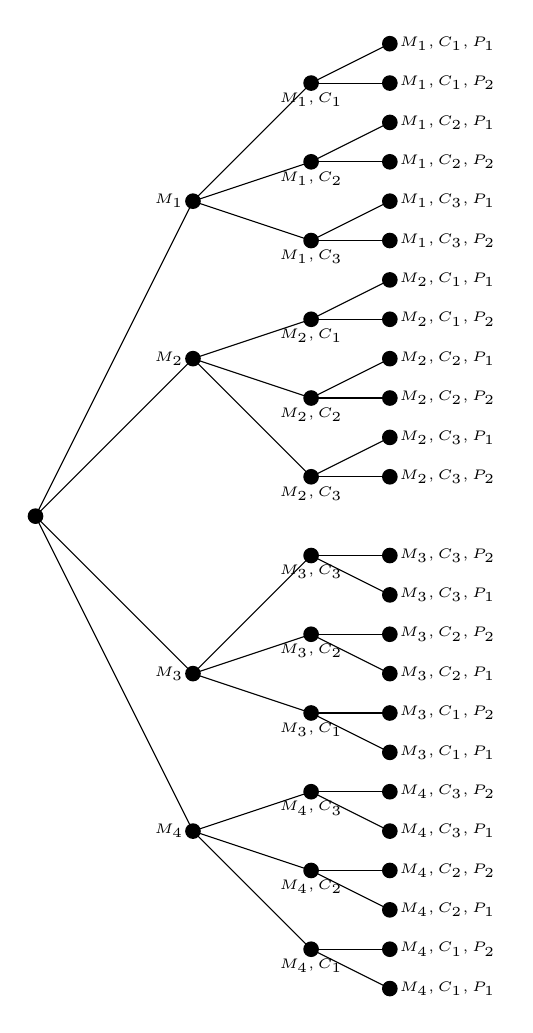
\begin{tikzpicture}[scale=0.5]
            \node at (0, 0)[circle,fill,inner sep=2pt]{};
            \foreach \m in {1,2,-1,-2}
            {
            \pgfmathparse{(\m>0) ? 1 : -1};
            \edef\direction{\pgfmathresult};
            \edef\my{\m*4};
            \node at (4, \my)[circle,fill,inner sep=2pt]{};
            \pgfmathparse{(\m>0) ? int(3-\m) : int(2-\m)};
            \edef\i{\pgfmathresult};
            \node[left] at (4, \my){\tiny $M_{\i}$};
            \foreach \c in {0,1,2}
            {
            \edef\cy{\m*6-5*\direction+\c*2*\direction};
            \node at (7, \cy)[circle,fill,inner sep=2pt]{};
            \pgfmathparse{int(3-\c)};
            \edef\j{\pgfmathresult};
            \node[below] at (7, \cy){\tiny $M_{\i},C_{\j}$};
            \foreach \p in {0,1}
            {
            \edef\dy{\cy+\p*\direction};
            \node at (9, \dy)[circle,fill,inner sep=2pt]{};
            \pgfmathparse{int(2-\p)};
            \edef\k{\pgfmathresult};
            \node[right] at (9, \dy){\tiny $M_{\i},C_{\j},P_{\k}$};
            \draw (9, \dy) -- (7, \cy);
            }
            \draw (7, \cy) -- (4, \my);
            }
            \draw (4, \my) -- (0, 0);
            }
        \end{tikzpicture}
    \end{center}

    从左到右阅读上图,我们就是在按照既定的三步过程进行。最左边的单个顶点代表过程的开始 --- 此时还没有做出任何决定。由该顶点延伸出的四条边代表我们可以选择的四门数学课程,每条边都标记着 $\mathcal{M}$ 的一个元素。无论选择哪条边(即哪门数学课程),下一个顶点都会延伸出三条边,代表我们可以选择的三门计算机课程,这些边标记着 $\mathcal{C}$ 的相应元素。接下来,每个顶点又延伸出两条边,标记着 $\mathcal{P}$ 的相应元素。

    这张图的好处在于,我们可以通过沿着边上的标签,准确地看到这个过程的 $24$ 种结果。例如,最右侧顶部的那个顶点,它对应于选择 $M_1, C_1$ 和 $P_1$;我们也可以将其表示为有序三元组 $(M_1, C_1, P_1)$。在该顶点的下方,我们会看到一个顶点对应于有序三元组 $(M_2, C_3, P_1)$。每个顶点都有一个有序三元组表示!当我们应用乘法原理时,实际上是在计算几个集合的\emph{笛卡尔积}的基数。这个过程就是识别组成集合的元素并将它们排列成一个有序元组。乘法原理告诉我们,通过计算所有这些元组组成的集合的基数,可以知道有多少种排列方式。在这个具体的例子中,我们有:
    \[|\mathcal{M} \times \mathcal{C} \times \mathcal{P}| = |M| \cdot |C| \cdot |P| = 4 \cdot 3 \cdot 2 = 24\]

    现在你觉得这种解释更清楚了吗?这是否更好地帮助你理解乘法原理的实际应用?
\end{example}

\subsubsection*{更正式的陈述}

请参见练习 \ref{exc:exercises8.9.1},该练习要求证明以下定理。这是乘法原理在数学上的更正式的表述。在陈述定理之后,我们将解释它与之前版本的关系。

\begin{theorem}[乘法原理(集合论版本)]\label{theorem8.2.10}
    设 $n \in \mathbb{N}$。假设 $\forall i \in \mathbb{N} \centerdot T_i$ 为有限集。则
    \[\Bigg|\prod_{i \in [n]} T_i \Bigg| = |T_1 \times T_2 \times \dots \times T_n| = |T_1| \cdot |T_2| \cdot \dots \cdot |T_n| = \prod_{i \in [n]} |T_i|\]
\end{theorem}

该定理与之前提到的乘法原理的关系如下。集合 $T_1$ 的元素代表在步骤 $1$ 中可以做出的选择。对于 $T_1$ 的每个元素,我们定义集合 $T_2$ 表示步骤 $1$ 做出选择\emph{之后},步骤 $2$ 中可以做出的选择。假设无论步骤 $1$ 的选择是什么,步骤 $2$ 中的选择数量都是相同的。因此,定理的结论只涉及 $|T_i|$ 是合理的,因为这个值是明确的。同理,$T_3$ 表示在步骤 $1$ 和 $2$ 之后步骤 $3$ 中可以做出的选择集合,假设 $|T_3|$ 也是明确的。

最终,我们可以用一个有序 $n$ 元组来描述这个过程的\textbf{输出},其中第 $i$ 个坐标是集合 $T_i$ 的一个元素。虽然该元素取决于之前的坐标,但其选择\textbf{数量}与之前的选择无关。因为我们最终只关心可能结果的\textbf{数量},所以这个结果是合理的。实际上,\textbf{列出}所有结果需要仔细分析每一步,看看特定选择如何影响下一步以及后续步骤的选择,但这不是结论的重点。这就是为什么,实质上,结果证明有限集的乘积大小等于它们大小的乘积。

\subsubsection*{示例:应用加法和乘法原理}

让我们来练习使用这两条原理。你会注意到,为了方便引用,我们会将这两条原理分别缩写为 ROS 和 ROP。没错,每次使用时,我们确实需要引用它们!\\

\begin{example}[车牌]
    假设车牌号字符串由 $6$ 或 $7$ 个字符组成,每个字符可以是字母 ($A$ 到 $Z$) 或数字 ($0$ 到 $9$)。
    \begin{enumerate}[label=(\arabic*)]
        \item 总共可以有多少张车牌?

              我们需要根据字符串的长度,分为 $6$ 位和 $7$ 位两种情况。

              对于每种情况,我们有一个 $6$ 步或 $7$ 步的过程。在第 $i$ 步,我们在字符串的第 $i$ 个位置填入 $36$ 个选项中的一个(包括 $26$ 个字母和 $10$ 个数字)。

              因此,根据 ROP,长度为 $6$ 的字符串有 $36^6$ 种可能,长度为 $7$ 的字符串有 $36^7$ 种可能。

              根据 ROS,总共有 $36^6 + 36^7$ 种车牌字符串。\\
        \item 有多少车牌最多只有一个数字?

              我们需要根据是否包含 $0$ 个数字或 $1$ 个数字来进行划分。
              \begin{itemize}
                  \item 如果没有数字,在每一步中我们都会在相应位置放置一个字母。根据 ROP,我们可能有 $6$ 个字母(产生 $26^6$ 种可能性)或 $7$ 个字母(产生 $26^7$ 种可能性)。

                        根据 ROS 计算,可能有 $26^6 + 26^7$ 种可能。
                  \item 如果包含 $1$ 个数字,首先在步骤 $1a$ 中选择哪个位置用数字填充,然后在步骤 $1b$ 中选择具体的数字,其余位置都用字母填充。

                        这种情况下,有 $6$ 或 $7$ 种选择哪个位置用数字填充,然后有 $10$ 种选择具体数字的方式,其他位置每个都有 $26$ 种选择。根据 ROS 和 ROP,我们得出有 $6 \cdot 10 \cdot 26^5$ 或 $7 \cdot 10 \cdot 26^6$ 种可能性。
              \end{itemize}
              综上,根据 ROS,我们一共有
              \[(26^6 + 6 \cdot 10 \cdot 26^5) + (26^7 + 7 \cdot 10 \cdot 26^6)\]
              种可能的结果。\\
        \item 有多少车牌至少有两个数字?

              我们可以像上面,将这组车牌分为包含 $3$ 位、$4$ 位、$5$ 位、$6$ 位和 $7$ 位数字的车牌。然后,我们需要计算每个集合的数量并将它们加起来。那么,含有 $4$ 位数字的车牌有多少呢?在 $6$ 个位置中选择 $4$ 个位置放数字,有多少种方法?这时候,二项式系数就派上用场了(在我们定义并推导出公式之后)。

              让我们复用刚才的工作成果!将所有车牌(集合 $Y$)分为最多 $1$ 位数字的车牌(集合 $X_1$)和至少 $2$ 位数字的车牌(集合 $X_2$)。注意这是一种划分,所以 ROS 告诉我们 $|Y| = |X_1| + |X_2|$。通过代数运算,我们得到想要的表达式是
              \begin{align*}
                  |X_2| & = |Y| - |X_1|                                                                       \\
                        & = (36^6 + 36^7) - [(26^6 + 6 \cdot 10 \cdot 26^5) + (26^7 + 7 \cdot 10 \cdot 26^6)]
              \end{align*}
              只需代入我们已经推导出的表达式即可。这样做非常方便!

              通常来说,这是一种有效的策略:为了计算一个集合的大小,我们可以先计算它的补集(即集合外的所有``其他''元素的集合),然后从``总数''中减去补集元素的数量。然而,需要注意的是,我们目前只能使用加法原理,还没有减法原理,所以我们应该始终小心地通过\emph{划分}和\emph{加法}来表达这个步骤。减法原理出现后,我们可以进行数字或代数变量的减法操作。最终,当我们的数学能力更强时,可以直接跳过这些形式化步骤,直接谈论``减去''一个数量;但目前,我们希望强调这些计数方法的基础,因此需要谨慎地使用加法原理并进行准确的措辞。\\
        \item 有多少车牌不包含元音字母和偶数数字?

              这种情况只是限制了每一步的选择数量。因为只有 $21$ 个字母和 $5$ 个数字可供选择,所以根据 ROP 和 ROS,我们可以得到
              \[26^6 + 26^7\]
              种可能的结果。
    \end{enumerate}
\end{example}